% ---------------------------------------------------------------------------
\section{Experiments}
\label{sec:experiments}

\subsection{Evaluation protocol}
\label{sec:eval}

\paragraph{Data and splits.}
We evaluate on DENTEX's official 50-image validation set (46 pathological images with 182
annotated target teeth, plus 4 healthy controls) as the test set, used exactly once for final
numbers. All configuration choices --- checkpoint selection, ablation conditions, group-size
sweeps --- are made on a fixed dev split of $\sim$70 training images drawn once with a fixed
seed, so that no choice leaks into the test result. Healthy images are evaluated with ground
truth $\emptyset$: an invented finding on a healthy image is charged to precision, which is
where it belongs. Cross-dataset context comes from the Tufts Dental Database
\citep{tuftsdatabase}, which contributes training traces and grounding training data but is not
used for test-time evaluation in this draft.

\paragraph{Metrics.}
Findings are matched as a \emph{set}: predictions and annotations are paired one-to-one by
optimal assignment \citep{kuhn1955hungarian}, and a finding is correct at two levels (exact:
right tooth and diagnosis; tooth-only: right tooth). Counts are pooled over all findings before
computing precision/recall/F1, so a healthy image's invented finding costs precision and images
with many findings are not diluted by averaging per-image scores. Uncertainty is quantified by
resampling whole \emph{images} (not findings) with replacement; comparisons between conditions
are paired, using the same resamples on the images the conditions share. Alongside accuracy we
report the fraction of healthy images on which findings were invented, the fraction of episodes
ending without a parseable answer, and expected calibration error (ECE) \citep{guo2017calibration}
between stated confidence and correctness.

\paragraph{Conditions.}
Every condition is a checkpoint (base, SFT, GRPO) with or without tool access, evaluated under
the input geometry used in training (original images for native-trained checkpoints; the
canonical views of \cref{fig:inputgeom} for canonically trained ones; tools always operate on
the native image) and additionally at original size. The no-tools arms use the \emph{same} SFT and GRPO recipe on the
1{,}847 single-turn traces, so tool contribution is not confounded with training recipe. \cref{fig:design} summarizes the
design.

\begin{figure}[tbp]
  \centering
  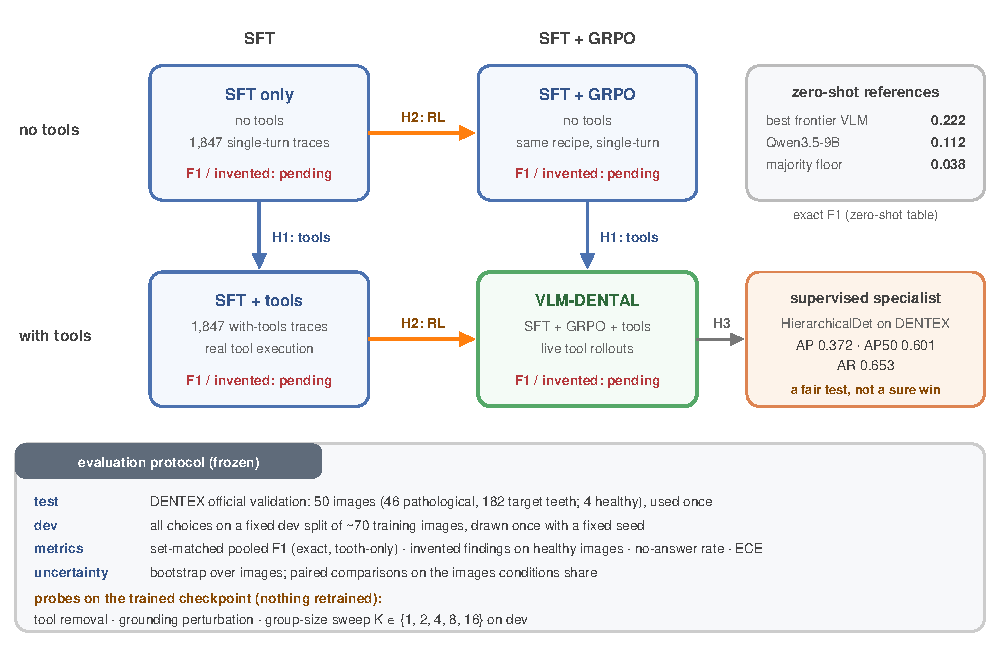
\includegraphics[width=\linewidth]{fig_design}
  \caption{Experimental design. The four conditions form a $2\times2$ (SFT vs.\ SFT$+$GRPO, with
  vs.\ without tools) trained with one recipe, so H1 (tools help) compares rows within a column
  and H2 (RL helps) compares columns within a row; H3 positions the full system against a
  supervised specialist, next to the zero-shot references of \cref{tab:zeroshot}. Result cells
  are pending the first hardware run, as in \cref{tab:main}; the protocol is frozen
  (\cref{sec:eval}).}
  \label{fig:design}
\end{figure}

\subsection{Zero-shot baselines: the case for looking again}
\label{sec:baselines}

\begin{table}[tbp]
  \centering
  \small
  \caption{Zero-shot frontier VLMs on the DENTEX validation set ($N=50$ panoramic radiographs;
  set-level matching over all annotated findings). Exact match requires the right tooth
  \emph{and} diagnosis. ECE = expected calibration error.}
  \label{tab:zeroshot}
  \begin{tabular}{lrrrrrr}
    \toprule
    Model & $N$ & FDI acc. & Exact acc. & Exact F1 & 95\% CI & ECE \\
    \midrule
    Moonshot Kimi-k3 & 50 & 64.0\% & \textbf{46.0\%} & \textbf{0.222} & [32.0, 60.0] & \textbf{0.214} \\
    Meta Llama 3.2 90B & 46 & 45.7\% & 37.0\% & 0.098 & [23.9, 52.2] & 0.395 \\
    Gemini 3.5 Flash & 50 & 62.0\% & 36.0\% & 0.188 & [22.0, 50.0] & 0.560 \\
    MiniMax M3 & 50 & 62.0\% & 32.0\% & 0.110 & [20.0, 44.0] & 0.493 \\
    Gemini 3.5 Flash Lite & 50 & 54.0\% & 32.0\% & 0.166 & [18.0, 46.0] & 0.596 \\
    Qwen3.5-9B (our backbone) & 49 & 53.1\% & 30.6\% & 0.112 & [18.4, 42.9] & 0.600 \\
    Majority-class floor & 50 & 38.0\% & 8.0\% & 0.038 & [2.0, 16.0] & -- \\
    Meta Llama 3.2 11B & 50 & 26.0\% & 4.0\% & 0.010 & [0.0, 10.0] & 0.678 \\
    \bottomrule
  \end{tabular}
\end{table}

\cref{tab:zeroshot} establishes the problem the agent architecture addresses. Even the best
frontier model misses more than half of the exact findings; the best-calibrated model still
carries ECE 0.21 while most models report 0.85--0.95 confidence on hallucinated positions; and a
dense 11B generalist falls \emph{below the majority-class floor}, a statistical collapse rather
than a graceful degradation. The failure modes are structural, not stochastic: quadrant
inversions from the OPG's left/right display convention, a resolution bottleneck that reduces an
early caries to a sub-patch blur, tissue-masking of periapical radiolucencies, and severe
overconfidence. Each of these maps onto a specific tool in \cref{tab:tools} --- which is the
design rationale of the suite, not a post hoc story: grounding corrects spatial disorientation,
\texttt{zoom\_crop} bypasses the resolution bottleneck, \texttt{window\_level} and
\texttt{enhance\_contrast} counter tissue masking, and \texttt{contralateral\_compare} tests
symmetry hypotheses before commitment.

\subsection{Main results}
\label{sec:mainresults}

\begin{table}[tbp]
  \centering
  \small
  \caption{Main results on the DENTEX validation set (pooled finding-level, set-matched);
  ``Best zero-shot frontier'' is the best row of \cref{tab:zeroshot}. Cells marked
  \todo{} are pending the first hardware training run; the experimental design and
  metric definitions are final and frozen (\cref{sec:eval}).}
  \label{tab:main}
  \footnotesize
  \setlength{\tabcolsep}{4pt}
  \begin{tabular}{@{}llccc@{}}
    \toprule
    Condition & Tools & Exact F1 $\uparrow$ & Tooth-only F1 $\uparrow$ & Invented$\downarrow$ \\
    \midrule
    Best zero-shot frontier & -- & 0.222 & -- & -- \\
    Zero-shot Qwen3.5-9B & -- & 0.112 & -- & -- \\
    Majority-class floor & -- & 0.038 & -- & -- \\
    SFT only (no tools) & -- & \todo{pending} & \todo{pending} & \todo{pending} \\
    SFT + tools & \checkmark & \todo{pending} & \todo{pending} & \todo{pending} \\
    SFT + GRPO (no tools) & -- & \todo{pending} & \todo{pending} & \todo{pending} \\
    \sys{} (SFT + GRPO) & \checkmark & \todo{pending} & \todo{pending} & \todo{pending} \\
    \midrule
    \multicolumn{5}{@{}l@{}}{Supervised specialist (HierarchicalDet), DENTEX: AP 0.372 / AP$_{50}$
    0.601 / AR 0.653 \citep{hamamci2024dentex}} \\
    \bottomrule
  \end{tabular}
\end{table}

\cref{tab:main} is the paper's primary claim table: does the agentic recipe beat zero-shot
inference and the same backbone without tools (H1: tools help; H2: RL helps), and where does it
stand against a supervised specialist (H3, framed as a fair test rather than a guaranteed win).
The training runs are in progress; all result cells are filled from the frozen evaluation
protocol above as runs complete.

\subsection{Mechanism analysis: does tiered perturbation elicit self-correction?}
\label{sec:mechanism}

Before any training, the corpus itself tests the central design claim of \cref{sec:perturbation}:
did the perturbation hook make the \emph{teacher} --- an expert-level frontier model with no
verbal hints --- actually inspect, judge, and correct grounding output, rather than scriptedly
nudge? We answer this by re-walking every with-tools trace (8{,}404 analysed
\texttt{locate\_tooth} returns) and reconstructing, for each located tooth, the box the teacher
was shown, the reference box, and every subsequent \texttt{nudge\_crop} applied to that box
through the trace. The shown box is recovered from the retained observation payloads (exact
post-perturbation boxes; validated at zero mean coordinate error against reference boxes on the
clean tier) or, where context truncation removed the observation, from the teacher's own
downstream \texttt{bbox} arguments, attributed by nearest center. Each attributed nudge is then
classified by direction: \emph{corrective} if its shift moved the working box toward the
reference center (cosine $>0.3$), \emph{away} if against it, \emph{rescaling} otherwise.

\begin{table}[tbp]
  \centering
  \small
  \caption{Correction behavior by perturbation tier, over the ground-truth-anchored subset of
  locate returns (reference box $=$ expert box; pathology cohorts). P(nudge) counts any
  attributed \texttt{nudge\_crop}; P(corrective) counts locates with at least one
  corrective-direction nudge; IoU after is over corrected locates. The clean tier is a control:
  with a correct box, corrective nudges are rare.}
  \label{tab:nudgetier}
  \begin{tabular}{lrrrrrr}
\toprule
Tier & $n$ & P(nudge) & P(corrective) & IoU before & IoU after & $\Delta$IoU \\
\midrule
none & 2,338 & 19.4\% & 1.1\% & 1.00 & 0.27 $\pm$ 0.18 & -0.73 \\
small & 1,337 & 23.1\% & 13.6\% & 0.45 & 0.45 $\pm$ 0.18 & -0.01 \\
big & 1,493 & 47.2\% & 38.4\% & 0.10 & 0.24 $\pm$ 0.18 & +0.15 \\
\bottomrule
\end{tabular}
\end{table}

\begin{figure}[tbp]
  \centering
  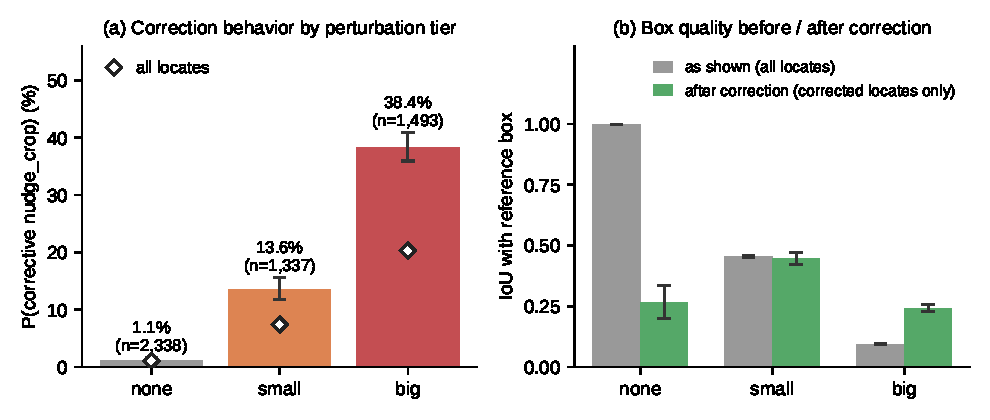
\includegraphics[width=\linewidth]{fig_nudge_tier}
  \caption{(a) Corrective \texttt{nudge\_crop} usage rises monotonically with perturbation
  severity on the ground-truth-anchored subset (bars, with Wilson 95\% intervals; the rates of
  \cref{tab:nudgetier}); diamonds give the same rate over all locate returns, including
  detector-anchored ones. (b) Mean IoU with the reference box as shown (over all locates with a
  recovered shown box) and after correction (over corrected locates only), with 95\% intervals
  of the mean; the two bars average different sets of locates, so their difference is not a
  paired gain. The ``none'' after-bar reflects the few corrective nudges on clean boxes
  (1.1\% of that tier), which are mostly reframing rescales rather than corrections.}
  \label{fig:nudgetier}
\end{figure}

\cref{tab:nudgetier} and \cref{fig:nudgetier} show the intended gradient, cleanly and
monotonically: corrective nudges on 38.4\% of large offsets, 13.6\% of small ones, and 1.1\% of
clean boxes. The clean-tier control matters: the teacher does not nudge reflexively --- with a
correct box it proceeds 98.9\% of the time, so the gradient is driven by the \emph{observed}
displacement, not a scripted habit. The small tier behaves exactly as designed as a judgment
call: nudges there are frequent (23.1\%) but only sometimes corrective (13.6\%), consistent with
the zoom margin often absorbing a small offset. On corrected large offsets, mean IoU against the
expert box improves from 0.095 to 0.243 per correction episode --- partial on average, because a
single nudge rarely lands perfectly --- with individual recoveries as large as IoU 0.066
$\to$ 0.938 on a DENTEX training image (\cref{fig:concept}; further episodes in \cref{fig:gallery}). The residual gap is not silently
absorbed: uncorrected spatial drifts are exactly what the verifier's third rejection category
(11 traces) caught and repaired during corpus construction.

Two further observations sharpen the picture. First, the split by reference type (full split in
\cref{app:mechanism}): on
\emph{detector-anchored} locates (exploratory calls during healthy-scan full-arch surveys, where
the reference is the detector's own box), correction is much rarer (5.0\% on large offsets vs.\
38.4\% ground-truth-anchored) --- during rapid systematic surveys the teacher surveys broadly
and does not inspect each exploratory box as carefully. We report this honestly; the
demonstrated skill this paper targets is the ground-truth-anchored pathology workflow. Second,
nudge \emph{rescales} skew small (scale $<1$): the dominant corrective pattern is
tighten-after-shift, matching radiologist behavior of zooming into a suspected lesion after
centering it.

\begin{figure}[!tb]
  \centering
  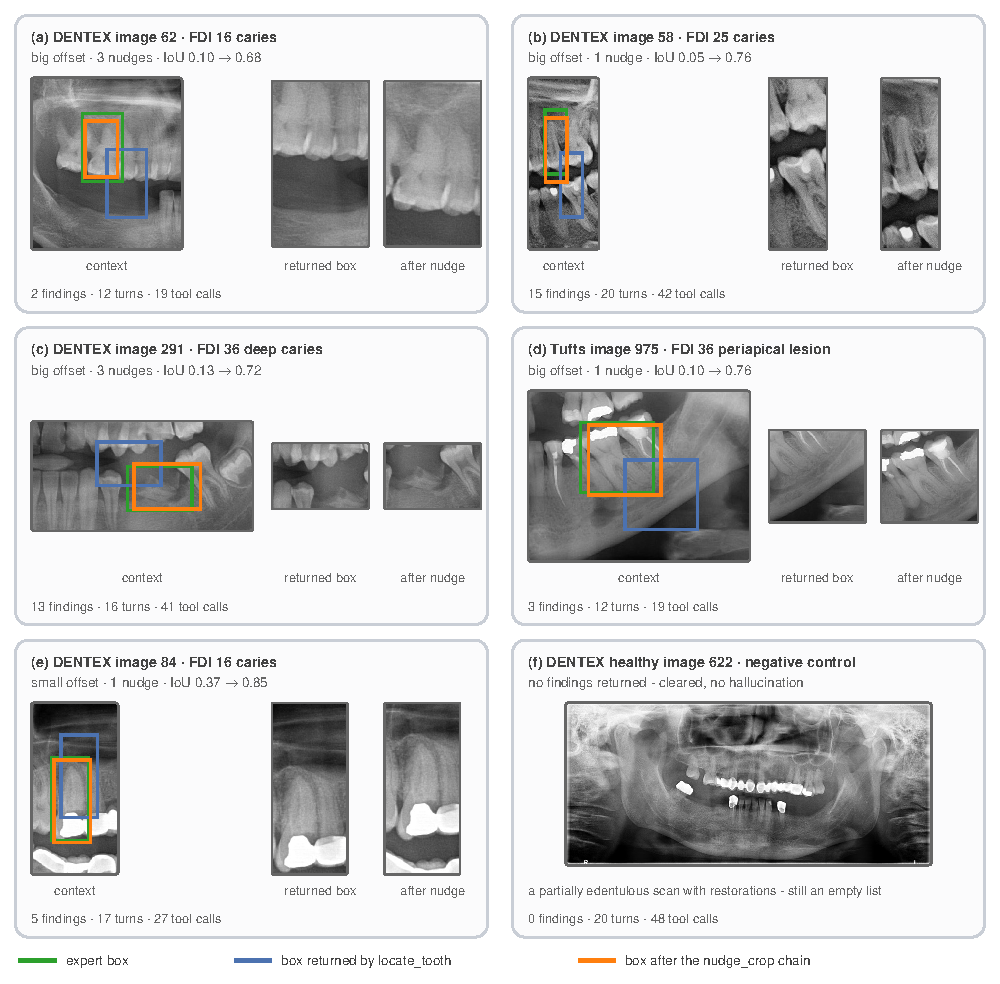
\includegraphics[width=\linewidth]{fig_gallery}
  \caption{Six verified with-tools episodes from the released corpus (five pathology, one healthy
  negative control), from two institutions. Each pathology panel shows the episode in context
  (expert box green, box returned by \texttt{locate\_tooth} blue, box after the
  \texttt{nudge\_crop} chain orange) and the crops the policy inspected before and after
  correcting; the header gives the offset tier, the number of nudges, and the IoU with the
  full-tooth expert box. (a) A three-nudge inspect--correct--re-inspect loop; (b) one nudge among
  15 findings and 42 tool calls; (c) a deep-caries tooth with a three-step chain; (d) a Tufts
  periapical lesion; (e) a small-offset judgment call; (f) a healthy scan cleared without a
  hallucinated finding. Tiers are recovered geometrically from the returned box (the
  perturbation metadata is stripped at release), and a policy that also rescales to focus can show a
  lower IoU than the displacement it recovered.}
  \label{fig:gallery}
\end{figure}

\subsection{Ablations and robustness checks}
\label{sec:ablations}

All ablation machinery is implemented and runs on a trained checkpoint with nothing retrained;
results are reported here as the runs complete.

\paragraph{Tool-removal probe.}
A tool is removed from the registry (absent from the prompt's tool list; calls to it return the
standard ``not recognized'' error), and we record both the score drop and how often the trained
agent attempts the missing tool. This measures dependence on each tool, including
\texttt{nudge\_crop}; because the checkpoint was trained with the tools present, it is a
dependence probe, not the score of a tool-free model --- the no-tools training arms in
\cref{tab:main} serve the latter role. \todo{pending}

\paragraph{Grounding-perturbation probe.}
Every \texttt{locate\_tooth} box at evaluation time is displaced by a fixed pseudo-random
fraction of its own size (the same wrong box for the same image and tooth across conditions, so
comparisons stay paired), and we report the IoU of the agent's working box against the annotated
tooth before and after its last \texttt{nudge\_crop}, plus how much of the annotated tooth the
last \texttt{zoom\_crop} actually shows. This is a stress test of the trained policy's
self-correction --- the deployed version of \cref{sec:mechanism}. \todo{pending}

\paragraph{Group-size sweep.}
GRPO group sizes $K \in \{1, 2, 4, 8, 16\}$ on the dev split, reporting pooled F1 per K with
paired comparisons and training cost; reports, never selects. \todo{pending}
